\documentclass[output=paper]{langscibook}
\ChapterDOI{10.5281/zenodo.6762278}

\author{Kendra V. Dickinson\affiliation{Rutgers University} and Glenn Martinez\affiliation{University of Texas at San Antonio}}
\title{Integrated assessment of Spanish heritage learners in a high school medical interpreter college/career program}
\abstract{Medical interpreters play an important role in bridging the language gap in health care and in reducing health disparities in minority language populations. The IMPACT (Interpreters for the Medical Profession through Articulated Curriculum and Training) program is a medical interpreter for Spanish Heritage Language (HL) speakers program at a career academy in central Ohio. The goals of this program include meeting the demand for language access in central Ohio while at the same time valuing HL learners’ experiences including language brokering (cf. \citealt{BurielMoran1998}), affirming their linguistic assets, and providing opportunities for them to develop competencies for future career and academic success. In this chapter, we report on the development, implementation, and evaluation of this program. We provide an integrated assessment approach that draws on qualitative and quantitative measures to highlight the role of program participation on students’ college and career readiness. Using a variety of methods including interviews, quantitative measures of career decision, and academic data, we demonstrate that participation in the IMPACT program positively influences students’ language proficiency, language attitudes, and career decision self-efficacy. In doing so, we provide a multi-faceted perspective on HL learner achievement that is consistent with the goals of HL education (\citealt{BeaudriePotowski2014}), that allows for integrated assessment of student development and career-readiness from a variety of different perspectives, and further demonstrates the importance of assessment models that consider the unique linguistic, social, and cultural assets of HL students.
\keywords{heritage, medical, interpreter, assessment, language}
}

\IfFileExists{../localcommands.tex}{%hack to check whether this is being compiled as part of a collection or standalone
  \addbibresource{../localbibliography.bib}
  % add all extra packages you need to load to this file

\usepackage{tabularx,multicol}
\usepackage{url}
\usepackage{soul}
\usepackage{longtable, xltabular}
\urlstyle{same}

\usepackage{listings}
\lstset{basicstyle=\ttfamily,tabsize=2,breaklines=true}

\usepackage{langsci-basic}
\usepackage{langsci-optional}
\usepackage{langsci-lgr}

\usepackage{todonotes}

\usepackage{makecell}

\usepackage{enumitem}
\usepackage{multirow}
\usepackage{langsci-branding}
\usepackage{langsci-gb4e}

  \newcommand*{\orcid}{}

\newcommand{\togglepaper}[1][0]{
%   \bibliography{../localbibliography}
    \papernote{\scriptsize\normalfont
    \theauthor.
    \titleTemp.
    To appear in:
    Change Volume Editor \& in localcommands.tex
    Change volume title in localcommands.tex
    Berlin: Language Science Press. [preliminary page numbering]
  }
  \pagenumbering{roman}
  \setcounter{chapter}{#1}
  \addtocounter{chapter}{-1}
}

% \newcommand{\keywords}[1]{\par\textbf{Keywords: #1}}

\renewcommand{\lsChapterFooterSize}{\footnotesize}

  %% hyphenation points for line breaks
%% Normally, automatic hyphenation in LaTeX is very good
%% If a word is mis-hyphenated, add it to this file
%%
%% add information to TeX file before \begin{document} with:
%% %% hyphenation points for line breaks
%% Normally, automatic hyphenation in LaTeX is very good
%% If a word is mis-hyphenated, add it to this file
%%
%% add information to TeX file before \begin{document} with:
%% %% hyphenation points for line breaks
%% Normally, automatic hyphenation in LaTeX is very good
%% If a word is mis-hyphenated, add it to this file
%%
%% add information to TeX file before \begin{document} with:
%% \include{localhyphenation}
\hyphenation{
anaph-o-ra
Dor-drecht
Ku-ka-ma
pre-dom-i-nant-ly
prog-ress
teach-er
Ri-ve-ra
}

\hyphenation{
anaph-o-ra
Dor-drecht
Ku-ka-ma
pre-dom-i-nant-ly
prog-ress
teach-er
Ri-ve-ra
}

\hyphenation{
anaph-o-ra
Dor-drecht
Ku-ka-ma
pre-dom-i-nant-ly
prog-ress
teach-er
Ri-ve-ra
}

  %\togglepaper[]
}{}
\shorttitlerunninghead{Integrated assessment of  heritage learners in a medical interpreter program}
\begin{document}
\shorttitlerunninghead{Integrated assessment of heritage learners in a medical interpreter program}
\maketitle

\section{Introduction}

Medical interpreters play a key role in bridging the language gap in health care and in reducing health disparities in minority language populations. Notwithstanding their crucial role in addressing language barriers, there is a national shortage of certified medical interpreters. A 2015 report from the Leonard D. Schaeffer Center for Health Policy and Economics at the University of Southern California found that there were only 738 certified medical interpreters in the state serving a population of 6.8 million Californians with limited proficiency in English (LEP, \citealt{Gonzales2015}). The present shortage, furthermore, will be exacerbated in the future as the Bureau of Labor Statistics predicts a 20\% increase in jobs for interpreters and translators by 2029 \citep{BureauofLaborStatistics2020}. The shortage of professional interpreters, as \citet{Dwyer2001} explains, is a community problem that requires a community-oriented and strengths-based solution \citep{Delgado-Romero2018}. Career and technical education (CTE) programs represent a significant community resource for addressing the shortage of medical interpreters.

 Current approaches to CTE differ significantly from earlier approaches commonly known as vocational education. As explained by \citet{BrandBrowning2013}, CTE “is eliminating vocational education that consisted of low-level courses, job training and single electives and replacing it with academically rigorous, integrated, and sequenced programs of study that align with and lead to postsecondary education” (\citeyear[2]{BrandBrowning2013}). The shifting demographics of CTE participation, moreover, present an unparalleled opportunity for the inclusion of medical interpreting in CTE targeted at Spanish heritage language (HL) learners. Within less than a decade, Latinx participation in all CTE in the United States has nearly tripled from a mere 757,952 participants in 2009--2010 to a total of 2,085,517 participants in 2016--2017 according to data available in the Perkins Data Explorer (\href{https://perkins.ed.gov/pims/DataExplorer}{{https:// perkins.ed.gov/pims/DataExplorer}}). Additionally, Latinx students accounted for only 9.9\% of the total number of CTE participants in 2009--2010, but that figure rose to 25\% by 2016-2017. These data suggest that Latinx students are gravitating towards CTE in greater numbers and that they are doing so at a pace that far exceeds other groups. CTE enrollments in health science cluster programs such as nursing, clinical lab sciences, and health information management, moreover, were the third most popular concentration options in 2016-2017. Between 2009--2010 and 2016--2017, enrollments in health science cluster programs grew 44\% and by 2016--2017 CTE concentrations in the health science cluster accounted for nearly 11\% of all CTE enrollments according to data available in the Perkins Data Explorer. These trends suggest that CTE programs may constitute an \textit{untapped pipeline} of medical interpreters to meet the health care needs of a growing LEP population and to simultaneously address the national shortage of certified medical interpreters.

In addition to the shifting demographics of CTE participation, programmatic changes also favor the inclusion of medical interpreting in CTE for HL learners. A significant opening for innovative curricula that span the high school/college/career pipeline has been created due to the following factors: (1) The reorganization of curriculum around clusters of occupations that share a similar knowledge and skill base, and (2) the formulation of career pathways that provide a coherent program of study blending high-level academics with technology applications and work-based learning \citep{CastellanoStone2003}. The evolving frameworks of Perkins legislation including the integration of academic and vocational education (Perkins II), the flexibility of state and local agencies to develop CTE programs (Perkins III), and the strengthening of connections between secondary and postsecondary education (Perkins IV) provide additional openings for the incorporation of medical interpreting in CTE \citep{Jocson2018}. Medical interpreting has been identified as a career specialty within the Support Services pathway of the Health Science Career Cluster \citep{AdvanceCTE2012}. Even so, few CTE programs have established medical interpreter training within their health science clusters.

This chapter reports on the development, implementation, and evaluation of a novel medical interpreter CTE program for Spanish HL learners established at a career academy in central Ohio. In doing so, we demonstrate an integrated assessment approach that draws on qualitative and quantitative measures to highlight the program’s impact on college and career readiness among Spanish HL learners. Much of the literature on HL assessment has focused on differentiating HL learners from second language (L2) learners and appropriately placing them in HL course sequences (\citealt{Thompson2015}; \citealt{PotowskiMorgan-Short2012}; \citealt{VergaraWilson2012}; \citealt{Fairclough2006}, \citealt{Fairclough2012a}; \citealt{Beaudrie2012}). Other research has focused on formative \citep{Carreira2012} and summative assessment \citep{ParraPolinsky2018} in Spanish HL courses and programs. An integrated assessment approach differs from these previous approaches because it provides a multi-faceted perspective on HL learner achievement that is consistent with the goals of HL education. \citet{BeaudriePotowski2014} propose the following seven HL education goals: language maintenance, acquisition or development of a prestige language variety, expansion of bilingual range, transfer of literacy skills, acquisition or development of academic skills, positive attitudes toward both the HL and various dialects of the language and its cultures, and acquisition or development of cultural awareness. The integrated assessment approach we adopt in this chapter seeks to provide a snapshot of HL learner achievement by focusing on multiple metrics that address these goal areas including language proficiency, academic performance, career self-efficacy (an individual’s belief that they can perform tasks and make decisions related to a career path: \citealt{TaylorBetz1983}), and ethnolinguistic identity. As described in more detail later in the chapter, we used a variety of instruments and metrics to piece together an overall profile of IMPACT participants. These included standardized tests, language proficiency assessments, self-efficacy instruments, and in-depth interviews with students. After a brief description of the IMPACT program and the setting where it was implemented, we will describe the specific methods used for the integrated assessment and present both the qualitative and quantitative findings.

\section{The IMPACT Program}

The IMPACT (Interpreters for the Medical Profession through Articulated Curriculum and Training) program is a high school-university-industry partnership designed to meet the demand for language access in the central Ohio region through a college and career readiness program for HL learners of Spanish. It creates a high school level pathway in medical interpreting to complement other health science CTE programs in Pre- and Multi-Skilled Nursing, Dental Technologies, and Medical Data Management. Along the way, students earn 12 college credits in Advanced Spanish, develop college readiness skills through mentoring, and gain experience in medical interpreting. The program consists of four phases, illustrated in \figref{fig:5:1}.

\begin{figure}
\caption{\label{fig:5:1}Four phases of the IMPACT Program}
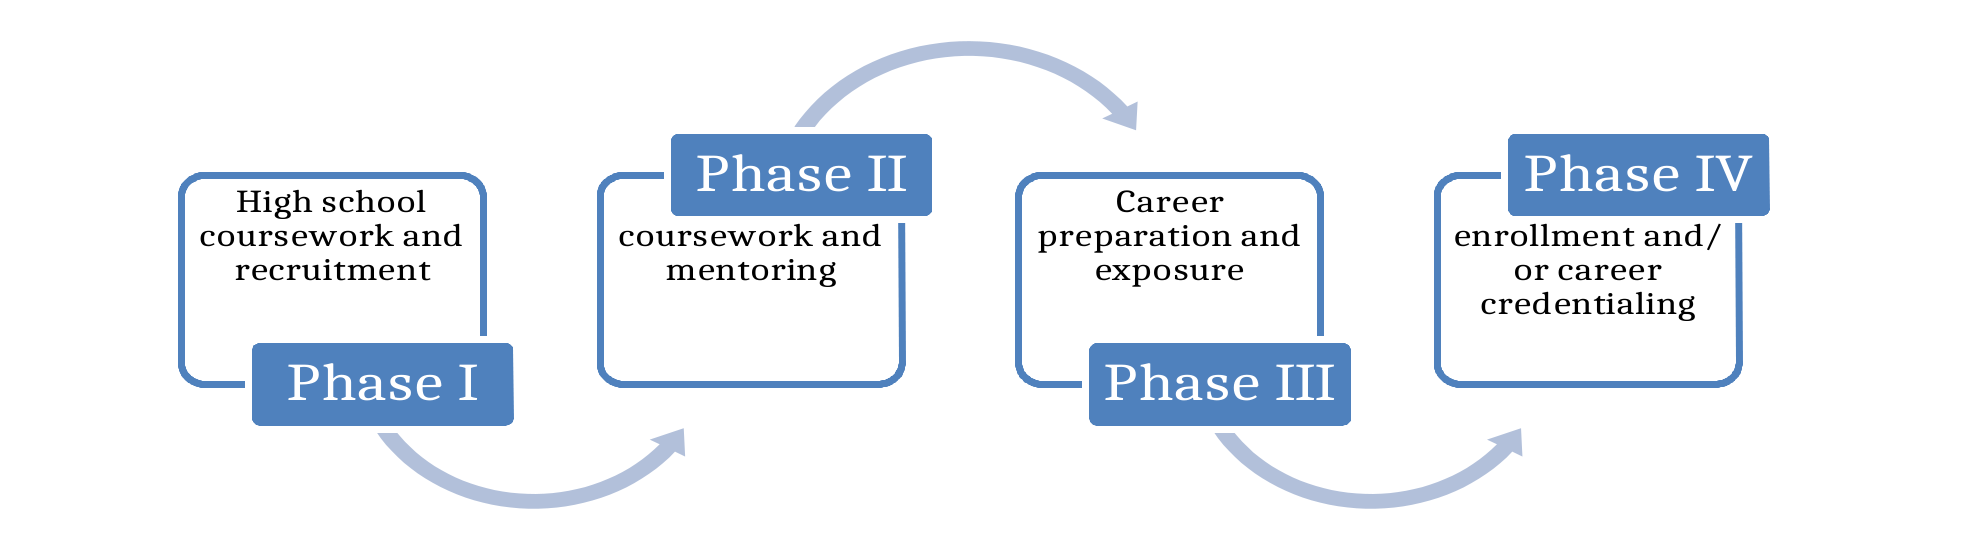
\includegraphics[width=\textwidth]{figures/rivera-fig-5-0.png}
\end{figure}

\textit{Phase 1} includes pre-program academic preparation and admission to the program. Students complete a two-year high school curriculum of Heritage Spanish during their freshman and sophomore years. Students who excel in these courses are identified by the Spanish teacher as potential candidates for the IMPACT program. Potential candidates are recruited to the program through a series of coordinated activities during the second semester of their sophomore year. The recruitment activities begin with an after-school information session including Spanish teachers, IMPACT program faculty and staff, and current or former IMPACT students. The information session covers the goal of the program, its structure and requirements, and the application process. Students who indicate interest in the program after the initial information session are invited to an evening meeting with their parents. At this meeting, IMPACT faculty and staff and high school counselors and administrators discuss the need for medical interpreters and bilingual health professionals in the central Ohio region and describe how the program will help students fill this need. Parents are also informed of the benefits and obligations of the state-sponsored College Credit Plus program. After the meeting with parents, students participate in an after-school application workshop in which university admissions officers are on hand to assist in completing their college application. \textit{Phase 2} consists of college level coursework. Upon admission to the university, students enroll in one advanced level Spanish course per semester for four semesters. The courses that students take are: Language, Culture and Communication in Latino Health (Spanish 2504); Advanced Spanish for Heritage Speakers (Spanish 3413); Translation and Interpreting in the Latino Community (Spanish 4369S); and Spanish in Health Care (Spanish 5201). \textit{Phase 3} consists of career preparation and exposure. In this phase, students complete The Community Interpreter (TCI®) interpreter training, a widely recognized curriculum for entry level interpreter training, and complete a 50-hour internship consisting of patient assistance and interpreter shadowing at a local hospital. \textit{Phase 4} consists of post-secondary education enrollment or entry into the profession. In this phase, students may enroll in college or sit for the National Board of Certification for Medical Intepreters (NBCMI) exam  or the Core Certification Healthcare Interpreter (CCHI) national medical exam. \tabref{tab:5:1} lists the activities included in the program and their alignment with the Knowledge and Skill Statements for the Support Services Pathway in the Health Science Career Cluster \citep{States’CareerClusterInitiative2008}.

\begin{sidewaystable}
\caption{\label{tab:5:1}Description of College and Career Activities in IMPACT}

\scriptsize
\begin{tabularx}{\textwidth}{@{}l@{}>{\raggedright}p{2cm}Q@{~}l@{~}p{7cm}@{}}
\lsptoprule
& Course & Course description & CTE & Knowledge and Skills Description\\
\midrule
\multicolumn{5}{l}{\textbf{College Coursework} }\\
\midrule
& \textbf{{Spanish 2504}{\slash}\newline{Communication 2704}} \textit{Language, Culture and Communication in Latino Health} & \multirow{1}{7cm}{Examines how language, culture and communication shape the healthcare experiences of Latinos in the US. Considers the individual and social factors contributing to health inequalities and key theories and techniques for developing health communication interventions.} & HLC05.01 & Healthcare workers will understand how their role fits into their department, their organization and the overall healthcare environment. They will identify how key systems affect services they perform and quality of care.\\

& \multirow{2}{2cm}{\textbf{Spanish 3413} \textit{Advanced Spanish for Heritage Learners}} & \multirow{2}{7cm}{Covers, reviews and practices grammatical structure through language, literature and culture of the Hispanic world as well as incorporates the experiences of heritage speakers in the US} & ESS01.02 & Demonstrate language arts knowledge and skills required to pursue the full range of post-secondary education and career opportunities.\\
&  &  & ESS02 & Use oral and written communication skills in creating, expressing and interpreting information and ideas including technical terminology and information.\\

& \multirow{2}{2cm}{\textbf{Spanish 4689S} \textit{Translation and Interpreting in the Latino Community}} & \multirow{3}{7cm}{This course introduces students to foundational concepts in translation and interpreting in community contexts among Latinos in the US. The course analyzes the theoretical, ethical and sociological dimensions.} & ESS03 & Solve problems using critical thinking skills (analyze, synthesize, evaluate) independently and in teams. Solve problems using creativity and innovation. \\
&  &  & ESS04 & Use information technology tools specific to the career cluster to access, manage, integrate and create information.\\
&  &  & IILC07 & Use leadership and teamwork skills in collaborating with others to accomplish organizational goals and objectives\\

& \textbf{Spanish 5201} \textit{Spanish in Health Care} & \multirow{2}{7cm}{Introduction to Spanish discourse about health and wellness within the cultural context of populations in the US and Latin America. Highlights the complex relationships between language, culture and power in discourse about health and wellness.} & IILC01.01 & Health care workers will know the academic subject matter required for proficiency within their area. They will use this knowledge as needed in their role.\\
&  &  & IILC02 & Use oral and written communication skills in creating, expressing and interpreting information and ideas including technical terminology and information. \\

\multicolumn{5}{l}{\textbf{Interpreter Training}}\\
\midrule
& \textit{The Community Interpreter ®} & \multirow{2}{7cm}{The Community Interpreter (TCI) is the leading national entry-level program to train intepreters to work in medical, educational and social service settings.} & HLC08 & Know and understand the importance of professional ethics and legal responsibilities.\\
&  &  & HLDP01.01 & Review, assess, differentiate and enhance the responsibilities of assigned roles and perform tasks safely following established internal and external guidelines in order to provide high quality effective support services in the health organization.\\
\lspbottomrule
\end{tabularx}
\end{sidewaystable}

The program was implemented at the South-Western~Career Academy (SWCA) which serves South-Western City School District in~Franklin County in central Ohio.~The Latinx population in Franklin County has grown 139\% since 2000. This county has the largest percentage of Latinx residents in the state representing 5\% of the total population~according to the Pew Research Center.~South-Western City School District serves the southwestern area of the City of Columbus and~the Columbus suburbs of Grove City and Galloway.~Latinx residents in the district make up between 8 and 20\% of the population. Latinx presence in the district represents 16.3\% of the total student population~according to the \citegen{OhioCTE2017} CTE Report Card for South-Western City School District.~SWCA~offers CTE~programs in 15 areas and, in 2018--2019,~enrolled a total~4,708 students from Westland High School, Franklin Heights High School, and Central Crossing High School. Approximately 16.7\% (796) of students at SWCA identify as Latinx.~Only 9\% of students at SWCA were classified as English Language Learners (ELL). Nearly half of the Latinx student population in the lower grades had exited the ELL program by the time they arrived at SWCA while maintaining strong Spanish language skills. SWCA offers four clinical concentrations in the health science cluster including~Medical Data Management, Multi-Skilled Nursing, Dental Technologies, and Pre-Nursing.~The total number of health science concentrations in these three programs is 174. A total of 58 students (33\%) identify as Hispanic, Latina/o or Latinx.

The IMPACT program began in 2016 and has enrolled a total of 31 students to date. A total of 20 students have completed the program and graduated from high school. All students who completed the program identified as Hispanic/Latinx. The majority of students were of Mexican origin and three students had ancestry in Peru, El Salvador, and Ecuador. 90\% of program completers (n = 18) graduated high school with an overall GPA of 3.0 or higher. Seventy percent of program completers (n = 11) have continued on to enroll in higher education and 35\% (n = 7) have received a full-ride scholarship to attend a four-year college or university. Twenty five percent of program completers (n = 5) have gone on to earn credentials or employment in the field of medical interpreting.

\section{Findings}

Our integrated assessment sought to gain an in-depth perspective of student achievement in and beyond the IMPACT program. In order to do so, we collected and analyzed data on a set of measures that align with the goals of HL education. These measures consisted of Spanish language proficiency assessed with the Parrot Language Proficiency Test, English language achievement assessed with the Ohio ELA test, academic achievement assessed with the College and Career Readiness (ACT) exam and high school grade point average (GPA), career decision making assessed with the Career Decision Self-Efficacy Scale, and ethnolinguistic identity and attitudes towards the HL assessed with in-depth individual interviews. In sum, our goal was to profile the IMPACT graduate in terms of language proficiency, language attitudes, and career decision making and at the same time compare the IMPACT graduate with other HL students with respect to academic achievement. Our integrated assessment approach thus sought to answer two research questions:

\begin{description}
\item[RQ1:] What is the profile of the IMPACT graduate with respect to language proficiency, language attitudes and career readiness?
\item[RQ2:] How do IMPACT graduates compare to non-IMPACT graduates with respect to academic achievement as measured by performance on the ACT exam and high school GPA?
\end{description}

\section{What is the profile of the IMPACT graduates?}

Previous research has shown that different factors can influence student academic outcomes and career and academic self-efficacy. Some of these influences include career pathway programs and career counseling \citep{StipanovicWitherell2017}, language brokering experiences \citep{BurielMoran1998}, student perception of barriers (see \citealt{LuzzoMcWhirter2001}; \textit{inter alia}), student support networks (e.g. teachers, friends, family; cf. \citealt{BerberyOBrien2018}; \citealt{CarpiLents2017}) and student linguistic and ethnic identity (\citealt{Mejia-SmithGushue2017}; \citealt{OjedaLeigh2012}). Traditional methods of assessment for HL learners often focus on tests, structured classroom activities, and analyses of HL production. Our integrated assessment approach sought to combine objective assessments of language proficiency and career decision making together with students' reflections on their own academic experiences, experiences in the IMPACT program, and their future careers. With this approach, we aimed to provide important insights into student learning and development outcomes.

\subsection{Language proficiency}

Thirteen IMPACT graduates took the Parrot Language Test (PLT). The PLT is a remote language testing system that measures functional abilities in the language based on the Interagency Language Roundtable (ILR) proficiency scale. The PLT uses multi-stimulus prompts including audio prompts, on-screen text and video accompaniment to generate evaluated speech. Results are based on agreement of three blind ratings that have been shown to achieve 90\% reliability \citep{ParrotND}. As a workplace language testing system, the PLT isolates three levels of workplace proficiency as follows:

\begin{itemize}[align=left, leftmargin=1.5cm, labelwidth=1.2cm]
\item[ILR 2] Limited Workplace Proficiency: speakers can handle routine interactions with a limited scope, describe objects and narrate events, and handle unanticipated complications.
\item[ILR 2+] Limited Workplace Proficiency Plus: speakers show fluency in specific areas of competence, describe and narrate with ample detail, and handle complications with ease.
\item[ILR 3] \begin{sloppypar}General Workplace Proficiency: speakers participate in extensive, sup\-ported discussion, manage unfamiliar workplace situations, and avoid errors that impact understanding.\end{sloppypar}
\end{itemize}

77\% percent (n = 10) of IMPACT graduates that took the PLT were certified at the ILR 3 level while 23\% (n = 3) were certified at the ILR 2+ level.

\subsection{Language attitudes and ethnolinguistic identity}

In order to explore language attitudes and ethnolinguistic identity among IMPACT graduates, we created a series of open-ended questions aimed at gaining insight into students’ future career and educational goals, career outlook, language use and identity, mentorship and role models, community, perceived barriers to success, and overall attitude towards the IMPACT program. We then set up conversational-style one-on-one interviews via Zoom between individual IMPACT students and their former Heritage Spanish high school teacher, organized around the questions that we created. Interviews lasted between 35--90 minutes, and students received a \$15 gift card as compensation for their participation. A total of 11 IMPACT graduates were interviewed.

The interview data pointed to substantive gains among HL students in terms of positive attitudes towards Spanish and cultural awareness of Latinx communities. Students interviewed described how participation in the program contributed to greater confidence in their language abilities and to a renewed sense of pride in their cultural heritage. In terms of language abilities, students commented that they no longer felt ashamed of their Spanish after participating in the IMPACT program. One student commented:

\begin{quote}
So, I would say like, in the interpreting thing-y, I would say like, I realized like, you know, I, I shouldn't be ashamed of speaking two languages. There's some people out there, that are just like, I don't know, they're just ashamed to speak the language. Cause there's like some Latino who like, they speak English and Spanish, but they're like embarrassed to speak Spanish, you know? I, I really don't care what people think.
\end{quote}

In terms of cultural heritage, on the other hand, students commented that they came out of the program with a greater appreciation for the variety of Latinx cultures in the U.S. For some students, this new appreciation led to a more positive perception of their own cultural heritage. One student put it this way:

\begin{quote}
Uh, I mean, uh, not gonna lie. Back then I was a little scared to say I was Salvadoran. 'Cause not a lot of people are Salvadoran, and there's like a lot of Mexicans. Now I'm not really scared to be like ``Oh, yeah, I'm from El Salvador.'' It's a little country, but it's there.
\end{quote}

Shifting attitudes about Spanish were not only reflected in students’ perception of themselves but also in their perception of the utility and value of the language in their future. One student commented on the economic advantage that he had because of his bilingualism:

\begin{quote}
We both have the same skills, but then here's one difference:  He speaks just English and I speak two. So, I have higher chance of getting hired than he would. Just like, small things like that, you know? That's reality. Um, it, it makes you look smarter, in some way, you know, just because, hey he speaks two languages, you know, he only speaks one. And it's, imagine if someday I would speak three languages, and it's like \ldots\,Wow. He's like super smart.
\end{quote}

Another student reflected on the cultural advantage of her bilingualism:

\begin{quote}
I feel like because I did this, I want to communicate more with people of all different types of, like all different types of Latinos, any part of like Latin America. I'd like to com- I would like to communicate with all of them and learn more about their traditions, their cultures, their music, their food, everything.
\end{quote}

Even while students commented on the positive benefits and advantages of bilingualism for themselves, they were equally emphatic about how their bilingualism would allow them to help others. One student commented: “I really like using Spanish, especially when it comes to helping others.” Another student expressed the same sentiment in greater detail:

\begin{quote}
And a bunch of like, Latinx people move to the United States because they want a better future for their children. Um, like the DREAM Act and all of that stuff. And, and there's this kinda p- pressure not to fail. But, at the same time, it's, it's, it's taking that dream and transforming it into your own. And how, like, my identity makes me want to do great things, because of my parents, you know? They sacrificed so much. I wanna do great things. But also, it, it allows me to go back and understand that the things that happened to me, I can shape them differently for another person, or I can help um, create uh, a social community, or uh, create this kind of community that helps our youth, and helps those that are now living through the problems today.
\end{quote}

Our interview data showed that IMPACT graduates emerged from the program with positive attitudes about their Spanish and greater awareness of the cultural variety of Latinx communities. At the same time, they emerged with a clear view of the advantages of being bilingual and with a commitment to using their bilingualism to help others.

\subsection{Career decision making}

Part of our integrated assessment also included a measure of career decision self-efficacy. Career decision self-efficacy has been shown to be related not only to career development among Latinx high school students, with respect to both vocational identity and career exploration activities, but also to student perception of barriers \citep{GushueScalan2006}. To measure levels of career decision self-efficacy among students in the IMPACT program, we utilized the Career Decision Self-Efficacy Scale-Short Form (CDSE-SF, \citealt{BetzTaylor2012}). In this instrument, students rated their degree of confidence in successfully completing 25 career-related tasks on a 5-point Likert Scale, where higher scores indicate higher levels of career decision-making self-efficacy. We administered the online version of the CDSE-SF to a total of 17 IMPACT graduates who elected to participate. Students were compensated with \$10 gift cards for their participation.

Items on the CDSE-SF are grouped into five principal areas: Goal selection, occupational information, planning, problem solving, and self-appraisal. \tabref{tab:5:2} below shows the average scores in these areas among this group of IMPACT students.

\begin{table}
\caption{\label{tab:5:2}Mean CDSE-SF Scores by area}
\begin{tabularx}{\textwidth}{Xrr}
\lsptoprule
 Topic & Mean (out of 5) & Standard Deviation \\
 \midrule
Self-appraisal & 4.02 & 0.60\\
Planning & 3.92 & 0.55\\
Goal selection & 3.90 & 0.61\\
Occupational information & 3.76 & 0.70\\
Problem solving & 3.76 & 0.60\\
\lspbottomrule
\end{tabularx}
\end{table}


This table shows that students scored, on average, between 3.76--4.02 in all areas targeted on the CDSE-SF.  Importantly, students scored, on average, above 3.5 in all areas, which is considered to indicate “Good confidence: Comfortable with this skill set” \citep{BetzTaylor2012}. However, there is slight variation among individual students, as shown in \tabref{tab:5:3}.

\begin{table}
\small
\caption{\label{tab:5:3}Distribution of CDSE-SF scores of HL students}
\begin{tabularx}{\textwidth}{l@{}YYY}
\lsptoprule
& { {Low to Little confidence: Needs intervention}} & {Moderate Confidence: May be comfortable exploring or may need some help} & {Good confidence: Comfortable with this skill set}\\
\midrule
& \textbf{1.0 to 2.5} & \textbf{2.5 to 3.5} & \textbf{3.5 to 5.0}\\
\midrule
{Self-appraisal} & { 0\%}

 (n = 0) & { 17.6\%}

 (n = 3) & { 82.4\%}

 (n = 14)\\
\tablevspace
{Planning} & { 0\%}

 (n = 0) & { 11.8\%}

 (n = 2) & { 88.2\%}

 (n = 15)\\
\tablevspace
{Goal selection} & { 0\%}

 (n = 0) & { 17.6\%}

 (n = 3) & { 82.4\%}

 (n = 14)\\
\tablevspace
{Occupational information} & { 5.9\%}

 (n = 1) & { 29.4\%}

 (n = 5) & { 64.7\%}

 (n = 11)\\
\tablevspace
{Problem solving} & { 0\%}

 (n = 0) & { 35.3\%}

 (n = 6) & { 64.7\%}

 (n = 11)\\
\lspbottomrule
\end{tabularx}
\end{table}

 Even though the majority of students scored within the highest bracket of scores (3.5--5.0) in all cases, there are cases in which students scored in the lower range. This breakdown allows us to identify areas in which students need additional support. For example, just one student scored within the 1.0--2.5 range in one area, occupational information. Using the CDSE-SF as an assessment metric for HL students would allow us to provide targeted intervention regarding career resources to this student in particular. Similarly, this method of assessment identifies the 11.8\%--35.3\% of students scored within the 2.5--3.5 range in all breakdown areas, allowing the IMPACT program to identify groups of students that need additional support and to provide interventions in those areas. Still, overall results show that students in the IMPACT program show good confidence levels in the areas targeted by the CDSE-SF, demonstrating that they are well-positioned for their future careers with regard to career decision-making self-efficacy.

\section{How do IMPACT graduates compare to non-IMPACT Latinx graduates?}

Another area of inquiry is the relationship between IMPACT program participation and student academic outcomes. In this analysis, we consider two conventional measures of student academic achievement: GPA and ACT exam scores. In our analysis, we find that Latinx students who participated in the IMPACT program were significantly more likely to have higher GPAs and ACT scores than Latinx students who did not participate in the program.

Data are drawn from students who took high school level Heritage Spanish I and II during the 2017--2018, 2018--2019, and 2019--2020 academic years. All students who were subsequently enrolled in the IMPACT program first took this course, but not all students who take the course ultimately enroll in the IMPACT program. Therefore, we are able to analyze the GPA and ACT scores of students who took the Heritage Spanish courses and did not enroll in IMPACT and students who did.

Along with student GPA and ACT scores, we also considered a number of additional factors as potential predictor variables. We considered students’ scores on \citet{Ohio’sStateTestsEnglishLanguageArtsandMathematicsPerformanceStandardsStandards2019} English Language Arts (ELA) tests 1 and 2 , taken in their freshman and sophomore years in high school, before enrollment in the IMPACT program, and student gender, school year, and IMPACT program participation as potential predictor variables.

In order to evaluate the potential relationships between IMPACT program participation and these metrics, data were examined and analyzed in R \citep{RCoreTeam2017} using the lme4 package \citep{BatesWalker2015}. First, we used a step-up method to build series of linear regression models of the data by sequentially added predictor, and then compared them using the ANOVA function in R to determine the best-fit models for our data.

\subsection{Student GPA}

Our first model compared the GPA scores of students who took the Heritage Language course and did enroll in IMPACT (n = 19) and those who took the course but did not enroll in IMPACT (n = 32). This model included student GPA as the dependent variable, and IMPACT program participation, school year, English Language Arts assessment 1 and 2, and student gender as potential predictor variables. The output of the best-fit model is shown in \tabref{tab:5:4} below.

\begin{table}
\caption{\label{tab:5:4} Best-fit model of student GPA}
\begin{tabularx}{\textwidth}{Xrrrrr}
\lsptoprule

&  & Estimate & Std. Error & t-value & p (> {\textbar}t{\textbar}) \\
\midrule
 & Intercept & 2.2955 & 0.1023 & 22.445 & <0.0001 \\
{Group}

\textit{(reference level = non-IMPACT)} & IMPACT & 1.3882 & 0.1676 & 8.285 & <0.0001 \\
\lspbottomrule
\end{tabularx}
\end{table}

The output shows the GPA of the students in the IMPACT group as compared to the GPA of the students in the reference level, the non-IMPACT group. None of the other factors considered were found to be statistically significant predictors of student GPA. The positive estimate for the IMPACT group (1.3882) shows that IMPACT students tended to have higher GPAs (mean = 3.7, standard deviation (sd) = 0.61) than non-IMPACT students (mean = 2.3, sd = 0.52). Furthermore, this difference is statistically significant, where IMPACT program participation significantly predicts higher GPA for those who participated in the program than for those that did not. This difference is visualized in the boxplot \figref{fig:5:2} below.

\begin{figure}
\caption{\label{fig:5:2}Boxplots of IMPACT vs. Non-IMPACT student GPA}
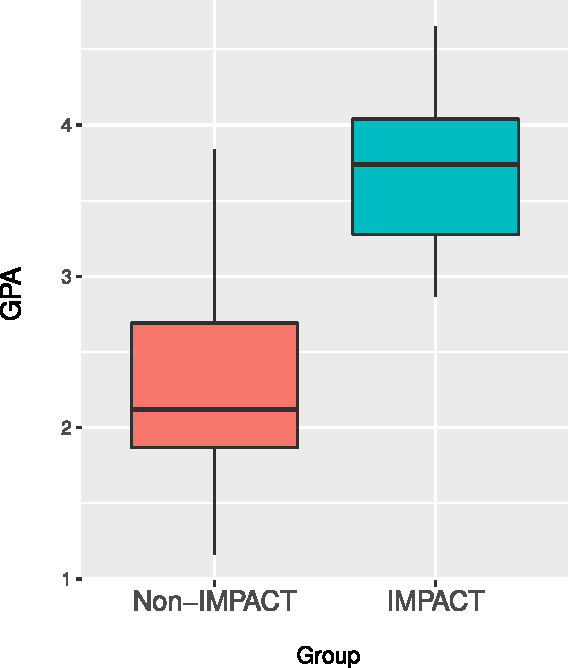
\includegraphics[width=.5\textwidth]{figures/dickinson-martinez-2.pdf}
\end{figure}


The potential influence of the IMPACT program on student GPA has far-reach\-ing implications. For example, in their study of Latinx high school students, \citet{BerberyOBrien2018} found that grade point average was the most influential factor in student college-going self-efficacy and educational goals. The IMPACT program motivates students to achieve higher GPAs in high school.

\subsection{ACT Scores}

Another conventional metric of academic achievement that we considered in the present analysis is student ACT score. For this analysis, we had access to ACT scores from 26 non-IMPACT graduates and 19 IMPACT graduates. For each student, the ACT score considered here is taken from a school administered, required test, taken by the student during their junior year. This model included student ACT as the outcome variable, and IMPACT program participation, school year, ELA assessments 1 and 2, and student gender as potential predictor variables. The output of the best-fit model is shown in \tabref{tab:5:5} below.

\begin{table}
\small
\caption{\label{tab:5:5}Best fit model of student ACT score}
\begin{tabularx}{\textwidth}{Qrrrrr}
\lsptoprule
&  & Estimate & Std. Error & t-value & p (> {\textbar}t{\textbar}) \\
\midrule
& Intercept & 21.2008 & 1.8582 & 11.409 & <0.0001 \\
{Group}

{\textit{(reference level = non-IMPACT)}} & IMPACT & 2.3034 & 0.8401 & 2.742 & <0.0001 \\
\tablevspace
{English Language Arts} & Limited & $-6.2503$ & {1.9714} & $-3.171$ & <0.01\\
Test 2 & {Basic} & $-5.3891$ & 1.6732 & $-3.221$ & <0.01\\
\textit{(reference level = Accelerated)}& {Proficient} & $-2.8584$ & 1.5836 & $-1.805$ & \textit{ns}\\
\tablevspace
{School Year} & {2018--2019} & $-2.8375$ & 0.8579 & $-3.308$ & <0.01\\
 \textit{(reference level = 2017--2018)} & {2019--2020} & $-1.9928$ & 1.1272 & $-1.768$ & \textit{ns}\\
\lspbottomrule
\end{tabularx}
\end{table}

 This output shows the statistical relationship between student ACT scores and IMPACT program participation, student ELA 2 assessment level, and school year. First, this output shows that IMPACT students were statistically significantly more likely to score higher on their ACT exam (mean = 18.47, sd = 2.94), than non-IMPACT students (mean = 14.65, sd = 2.82). Another significant predictor of student ACT scores shown above is the ELA 2 test score. This test is administered to students in their sophomore year of high school, as part of requirements established by the Ohio Department of Education, though this assessment has since been eliminated for future students \citep{EliminationofEnglishLanguageArtsIStateAssessment:InformationforDistrictsandSchoolsSchools2019}. The ELA tests have 5 potential levels of achievement, which are, in order of lowest to highest: Limited, Basic, Proficient, Accelerated, and Advanced. Students in the current sample achieved only the first four levels. The model output above shows that students who achieved “Limited” and “Basic” proficiency scores on their ELA 2 exam also scored significantly lower on their ACT exam than did students who received a rank of “Accelerated.” Furthermore, students who received a “Proficient” level on their ELA 2 exam did not receive ACT scores significantly different from those who achieved a rank of “Accelerated.” Releveling of the factors in the model revealed that the ACT scores received by students who scored “Limited” and “Basic” on their ELA 2 exam were not significantly different from each other. These differences are visualized in \figref{fig:5:3} below.

\begin{figure}
\caption{\label{fig:5:3}Boxplot of student ELA 2 scores}
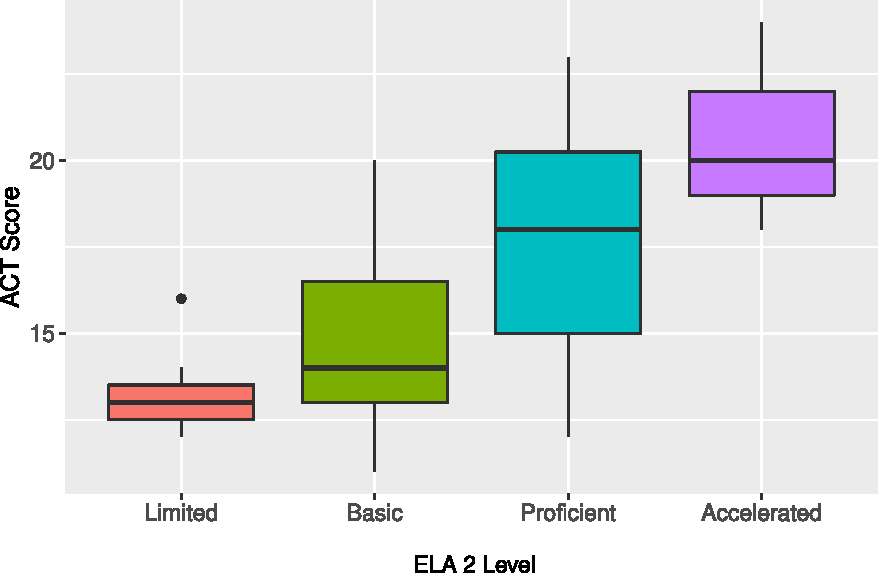
\includegraphics[width=.8\textwidth]{figures/dickinson-martinez-3.pdf}
\end{figure}

Finally, there is also a main effect of school year in these data. ACT scores for the group of students that we have data for were significantly lower in the 2018--2019 school year than they were for the 2017--2018 and 2019--2020 school years. There may be real-world explanations for this observation, such as the conditions under which the exams were administered, or this may simply be an outlying year.  Overall, these results illustrate that IMPACT program participation is the strongest predictor of ACT scores for this group of HL students, and that ELA 2 tests scores and school year also play a role in these outcomes.

\subsection{IMPACT student changes in ACT scores}

Because students take the school district-administered ACT exam during their junior year, many students will take the exam again. Therefore, we were able examine changes in ACT score for a subset of IMPACT students for whom the data was available (n = 16). Their first scores are from the ACT exam taken during their first year of participation in the IMPACT program, while their second scores are from their second year in the program.

In order to conduct paired t-tests on the data, we first needed to ensure normal distribution, due to the small sample size, using a Shapiro-Wilk test of normality \citep{ShapiroWilk1965}. Outputs of this measure show that neither students' first ACT score (p = 0.2659) nor students’ last ACT scores (p = 0.3635) were significantly different from normal distributions. This allowed us to more confidently conduct paired t-tests on the data. We then conducted a paired t-test to compare the means of two related samples, the students’ first and last ACT scores. The output of this test shows a significant difference between the two (t = $-2.6379$, df = 15, p-value = $0.01864$), where students achieved significantly higher scores on their last ACT exam than on their first. This difference is visualized in \figref{fig:5:4} below.

\begin{figure}
\caption{\label{fig:5:4}Boxplot of IMPACT student first and last ACT scores}
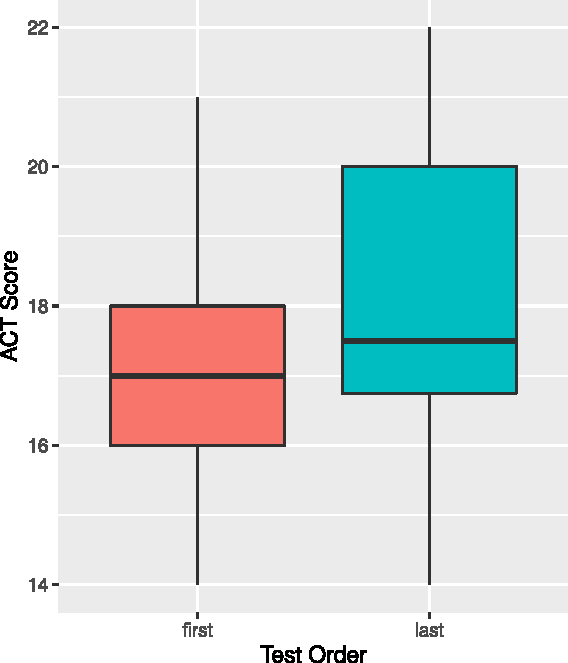
\includegraphics[width=.5\textwidth]{figures/dickinson-martinez-4.pdf}
\end{figure}

Furthermore, it is also of interest to examine how the ACT scores of individual students differ from their first to their last ACT exam. \figref{fig:5:5} below shows individual plots by student tracking the change between their first and their last ACT scores. From this image, we can see that the majority of individual students (68.75\%, n~=~11) scored better on their second ACT exam, whereas only 25\% (n~=~4) received the same score on both exams, and 6.25\% (n~=~1) received a lower score on their second exam.

\begin{figure}
\caption{\label{fig:5:5}IMPACT student first and last ACT score by student}
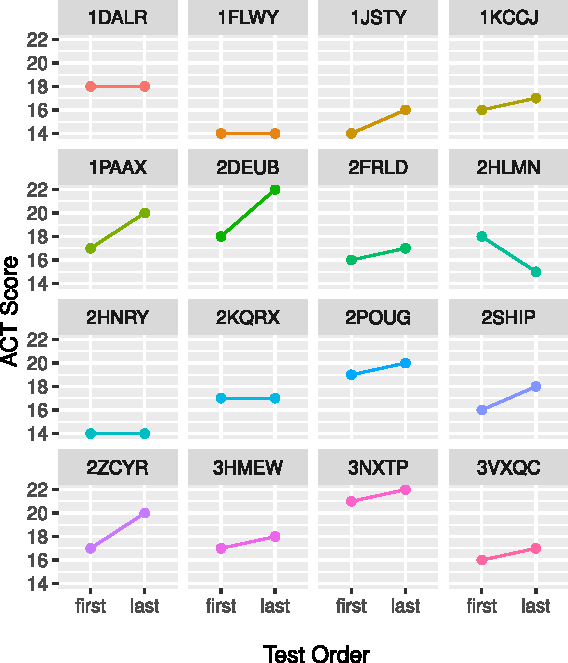
\includegraphics[width=.6\textwidth]{figures/dickinson-martinez-5.pdf}
\end{figure}


\section{Conclusion}

In this chapter, we have demonstrated an integrated assessment approach that draws on qualitative and quantitative measures to highlight the program’s impact on college and career readiness among Spanish HL learners. As opposed to focusing on differentiating HL learners from L2 learners, we have provided a multi-faceted perspective on HL learner achievement that is not only consistent with the goals of HL education, but that also allows for an integrated assessment of student development and career-readiness from a variety of different perspectives.

First, we have shown that language proficiency, language attitudes, and career decision self-efficacy were affected by participation in the IMPACT program. IMPACT students demonstrated high performance on a workplace language proficiency assessment. At the same time, students indicated more positive attitudes to Spanish and were able to make explicit connections between Spanish language proficiency and career opportunities. Second, we have shown that measures of career-decision self-efficacy, in this case the CDSE-SF, can be useful measures of career-readiness that can also allow the program to identify areas of student need and implement appropriate interventions. Third, we have shown the participation in a program like IMPACT has the potential to affect student outcomes in academic areas. For example, graduates of the IMPACT program had statistically significantly higher GPAs and ACT scores than HL students who did not participate in the program. We also saw the ACT scores generally increased for students after enrollment in the IMPACT program.

The student outcomes reported in this study reflect an innovative approach to heritage language teaching that connects language and culture to an obvious and immediate community need. By exposing heritage learners to the medical interpreting profession in a CTE context early in their schooling careers, students are given an opportunity to tap into cultural and linguistic funds of knowledge in a way that is often not available in mainstream CTE or Spanish language classes. The integrated assessment approach described in this chapter demonstrates the multiple effects that participation in this program had on academic, career and linguistic outcomes.

Our integrated assessment approach provides insights into the synergies between linguistic, academic, and career development of HL students and shows how this combined achievement interacts with affective dimensions of HL learning including the development of positive attitudes about Spanish and confidence in the advantages that the HL will provide in the students’ future career. We believe that innovative college and career oriented programming together with continuous integrated assessment can more effectively connect heritage language instruction with student success and thus contribute to a robust evidence base demonstrating the immense value of HL learning for Latinx students.


{\sloppy\printbibliography[heading=subbibliography,notkeyword=this]}
\end{document}
